\subsection{Software} \label{kap:Software}

Die Software des Planting Robots ist in der Programmiersprache C geschrieben und läuft auf dem ARM Cortex M0+ Mikrocontroller von NXP welcher auf dem FRDM-Board KL25Z (siehe Abb. \ref{fig:FRDM-KL25Z}) bestückt ist. Das FRDM-Board wird verwendet, weil damit schon im Modul PREN Erfahrungen gesammelt werden konnten. Ausserdem wird im Programmier-Modul INTRO auf Basis der Kinetis Mikrocontroller Familie Software entwickelt.

\begin{figure}[H]
	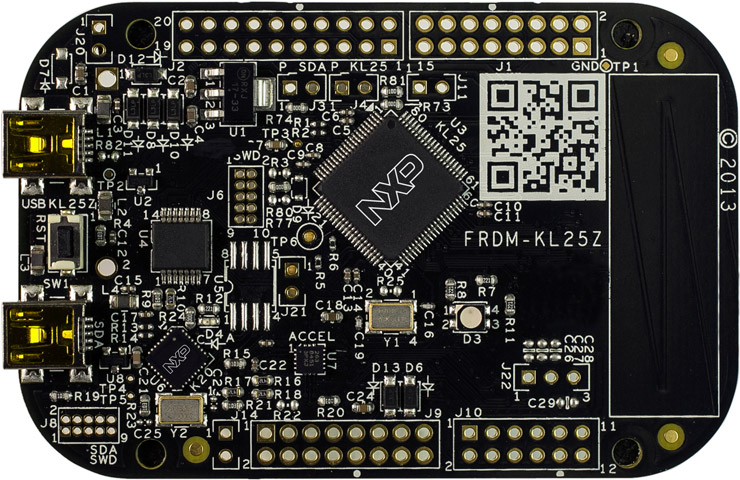
\includegraphics[width=0.6\textwidth]{Illustrationen/5-Konzept/FRDM-KL25Z.jpg}
	\caption{Software, FRDM-KL25Z \protect\cite{NXP}}
	\label{fig:FRDM-KL25Z}
\end{figure}

Als Betriebssystem dient das Real Time OS FreeRTOS. Vorteile von FreeRTOS gegenüber anderen C Betriebssystemen sind:

\begin{itemize}
	\item Seine geringen Ressourcenanforderungen an RAM, ROM und CPU Leistung. 
	\item FreeRTOS ist weit verbreitet und wird an der HSLU in diversen Softwareprojekten verwendet.
	\item Es ist absolut kostenfrei, auch für kommerzielle Anwendungen.
	\item FreeRTOS ist einfach in der Anwendung und eignet sich auch für grössere Projekte.
\end{itemize}

Die wichtigsten Softwarekomponenten sind in Abb. \ref{fig:Software_Uebersicht} abgebildet. Die Übergeordnete Softwarekomponente FSM implementiert eine State Machine, welche den Ablauf der Software steuert. Sie wird in einem Task realisiert. Hierarchisch untergeordnet befinden sich die Driver Komponenten. Sie bilden die Schnittstelle zur Hardware. Die Low Level Anbindung der jeweiligen Hardware Komponenten über Digital I/Os, UART, I$_{2}$C und Analog Inputs wird mit Processor Expert Komponenten realisiert. PE Komponenten erleichtern die Konfiguration von Peripherie-Registern des uC und bieten zusätzlich diverse C Methoden für die Verwendung genannter Peripherie. 

\begin{figure}[H]
	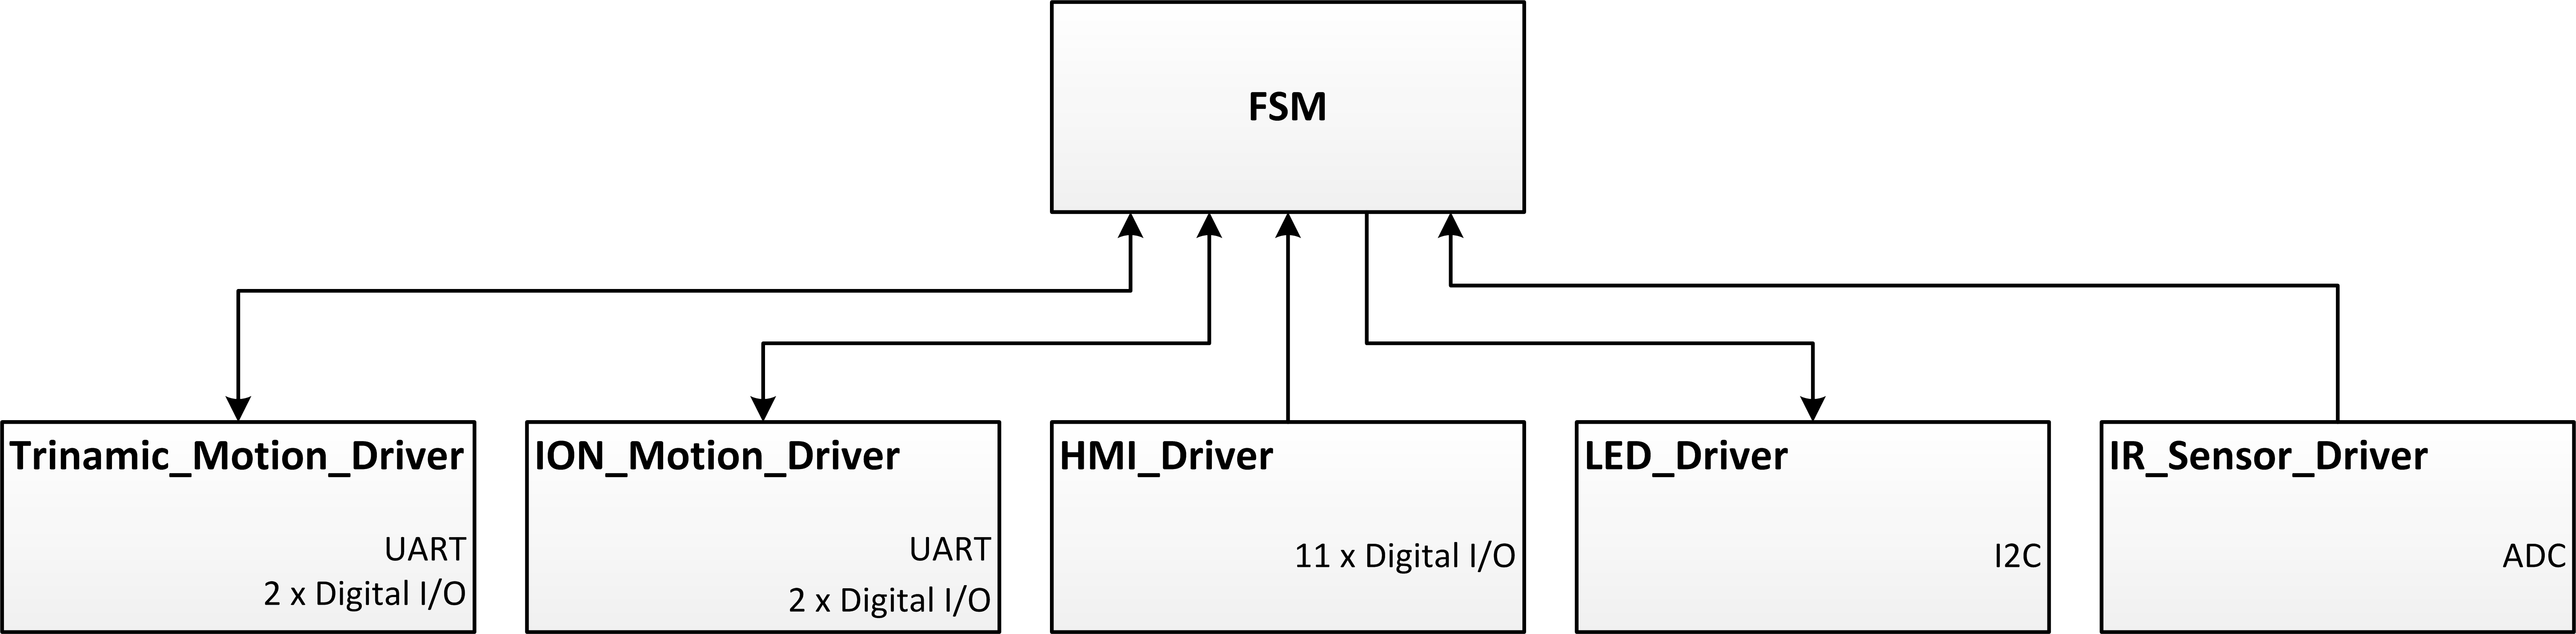
\includegraphics[width=1\textwidth]{Illustrationen/5-Konzept/Software_Uebersicht.png}
	\caption{Software, Übersicht Software Komponenten}
	\label{fig:Software_Uebersicht}
\end{figure}

Die verwendeten PE Komponenten sind in der Abb. \ref{fig:Software_Uebersicht} innerhalb der Driver Module jeweils rechtsbündig aufgelistet (UART, Digital I/O,...). Im folgenden Abschnitt werden die Driver Module kurz erklärt:

\begin{itemize}
	\item \textbf{Trinamic\_Motion\_Driver:} Steuert den BLDC Motoren Controller von Trinamic. Die Kommunikation wird über UART realisiert. Zwei Digital Outputs werden verwendet um die 36V Speisung und das Not Stop Signal des Motorentreibers zu schalten.
	\item \textbf{ION\_Motion\_Driver:} Steuert den 2 Kanal DC Motoren Controller von ION. Die Kommunikation wird über UART realisiert. Mit dem Digital Output Signal wird das 12V Relais auf dem Mainboard PCB für die Speisung des Treibers geschaltet.
	\item \textbf{HMI\_Driver:} Wertet die Taster des HMIs via Polling inklusive Software Entprellung aus. Die Taster sind über Digital Inputs direkt mit dem uC verbunden. Dieser Driver ist in einem Task realisiert.
	\item \textbf{LED\_Driver:} Steuert über die I$_{2}$C Schnittstelle das LED Treiber IC an. Für das pulsieren der LEDs wird ein Task erstellt.
	\item \textbf{IR\_Sensor\_Driver:} Implementiert die Messung sowie die Auswertung der IR-Sensor Daten zur Topferkennung. Die Topferkennung läuft dabei in einem Task.
\end{itemize}

Detailiertere Informationen zur implementierung der Software finden sich im Kapitel \ref{sec:Software}